\newpage
\section{Suggested solutions: $Z$-transform}

\begin{enumerate}
\item Given a discrete time signal $x[n]$, then the $z$-transform is defined as:
$$X(z)=\sum_{k=-\infty}^{\infty}x[k]z^{-k}.$$

\begin{enumerate}[a)]

\item Using the definition, we have:
$$X(z)=\mathcal{Z}\{\delta[n]\}=\sum_{k=-\infty}^{\infty}\delta[k]z^{-k}=\delta[0]z^{-0}=1,$$
since the impulse function is only non-zero for $n=0$, for which the value is $1$. 

\item The $z$-transform is linear and for a time-shift, we then have:
\begin{align*}
    X(z)&=\mathcal{Z}\{2\delta[n+4]\}=2\mathcal{Z}\{\delta[n+4]\}, \\
    &=2\sum_{k=-\infty}^{\infty}\delta[k+4]z^{-k}, \\
    &=2z^{4}\mathcal{Z}\{\delta[n]\}, \\
    &=2z^{4},
\end{align*}
since by the previous exercise $\mathcal{Z}\{\delta[n]\}=1$.

\item The $z$-transform of $h[n]=-41\delta[n-42]$ is done in the same way as the previous problem. Skipping the details, we obtain:
$$X(z)=\mathcal{Z}\{-41\delta[n-42]\}=-41z^{-42},$$
again by linearity and the time-shift theorem.

\item For $h[n]=\delta[n+1]-2\delta[n-1]+4\delta[n-4]$ we obtain again by linearity and the time-shift property:
$$X(z)=\mathcal{Z}\{h[n]\}=z-2z^{-1}+4z^{-4}.$$
\end{enumerate}

\item Let the system function for an LTI system be $\mathcal{H}(z)=z^{1}+1+3z^{-1}-0.5z^{-2}+4z^{-10}$.

\begin{enumerate}[a)]

\item If the system function is defined as above, then the impulse response is found by taking the inverse $z$-transform of $\mathcal{H}(z)$. We get:
$$h[n]=\delta[n+1]+\delta[n]+3\delta[n-1]-0.5\delta[n-2]+4\delta[n-10],$$
from this we conclude that the difference equation for the system is:
$$y[n]=x[n+1]+x[n]+3x[n-1]-0.5x[n-2]+4x[n-10],$$
since every LTI system can be expressed as a convolution of the form:
$$y[n]=h[n]*x[n]=\sum_{k=-\infty}^{\infty}h[k]x[n-k],$$
with $h[n]=\mathcal{T}\{\delta[n]\}$. 

\item In Listing \ref{code17_2} is a simple program to plot the impulse response for this system. 
\begin{lstlisting}[language=Python, caption=Code to plot the impulse response function,label=code17_2]
import numpy as n
import matplotlib.pyplot as plt

# sample value we want to plot on
nn = n.array([-2,-1,0,1,2,3,4,5,6,7,8,9,10])

# values for the impulse response function
h = n.array([0,1,1,3,-0.5,0,0,0,0,0,0,0,4])

# plot as a stem plot to emphasize the 
# discrete nature of the function
plt.stem(nn,h)
plt.xlabel("samples [n]")
plt.ylabel("$h[n]$")
plt.title("Impulse response")
plt.show()
\end{lstlisting}
The impulse response plot is shown in Figure \ref{fig17_2}.
\begin{marginfigure}
    \centering
    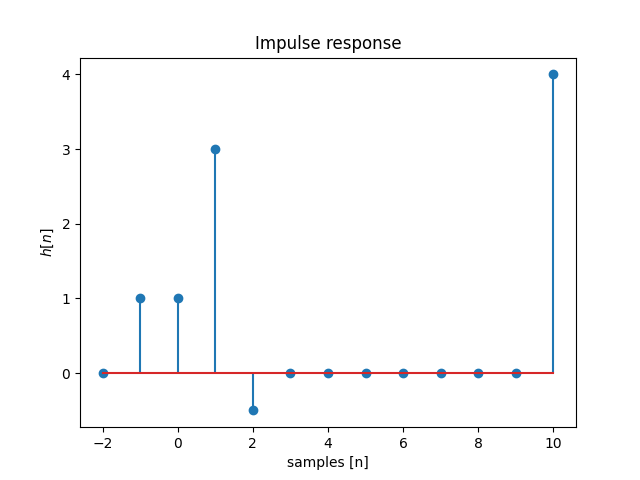
\includegraphics[width=7.5cm,height=7.0cm]{ch18/figures/17_2.png}
    \caption{Output of Listing \ref{code17_2}}
    \label{fig17_2}
\end{marginfigure}

\item If we define a new signal $y_{2}[n]=y[n-2]$, then by the time-shift theorem we have that the new system function will be:
$$Y_{2}(z)=z^{-n_{0}}\mathcal{H}(z)=z^{-2}\mathcal{H}(z)=z^{-1}+z^{-2}+3z^{-3}-0.2z^{-4}+4z^{-12},$$
this new system function will describe a system that is delayed by 2 samples compared to $\mathcal{H}(z)$.
\end{enumerate}

\item Let the system function of a discrete-time LTI system be defined as:
$$\mathcal{H}(z)=(z-e^{i\pi/4})(z-e^{-i\pi})z^{-2}.$$

\begin{enumerate}[a)]
\item To determine the effect of this system, factor it:
$$\mathcal{H}(z)=z(1-e^{i\pi}z^{-1})z(1-e^{-i\pi}z^{-1})z^{-2}=(1-e^{i\pi/4}z^{-1})(1-e^{-i\pi}z^{-1}).$$
Then we can view the system function as a cascade of two elementary systems of the form:
\begin{align*}
    \mathcal{H}_{1}(z)&=1-e^{i\pi/4}z^{-1},\\
    \mathcal{H}_{2}(z)&=1-e^{-i\pi}z^{-1}.
\end{align*}
This filter blocks sinusoidal signals where $\alpha_{1}=e^{i\pi/4}$ and $\alpha_{2}=e^{-i\pi}$, which correspond to normalized angular frequencies of $\hat{\omega}=\pi/4$ and $\hat{\omega}=-\pi$.

\begin{marginfigure}[-5cm]
\begin{center}
\begin{tikzpicture}
	\begin{axis}[axis equal, ymin=-1.5,xmin=-1.5,ymax=1.5,xmax=1.5,  ticks=none,
    xlabel=$\mathrm{Re}(z)$,
    ylabel=$\mathrm{Im}(z)$, axis lines = middle, width=7cm, height=7cm]
	\addplot [gray,domain=0:2*pi,samples=50]({cos(deg(x))},{sin(deg(x))});

\addplot [blue, mark = o,mark size=3pt] coordinates {({cos(45)}, {sin(45)})} {};   
\addplot [blue, mark = o,mark size=3pt] coordinates {({cos(180)}, {sin(180)})} {};  
\addplot [red, mark = x,mark size=3pt] coordinates {({0}, {0})} {}; 
\end{axis}
\end{tikzpicture}
\end{center}
\caption{The zeros of the system function $\mathcal{H}(z)$,
have $\alpha_k=\{e^{i\pi/4},e^{-i\pi}\}$. Zeros are marked with blue
    circles and poles are marked with red crosses.}
\label{z:ex3}
\end{marginfigure}

\item The poles and zeros of the system function are shown in Figure \ref{z:ex3}. 

\item The following code snippet will plot the magnitude response corresponding to $\mathcal{H}(\hat{\omega})=\mathcal{H}(z)|_{z=e^{i\hat{\omega}}}$:
\begin{lstlisting}[language=Python,caption=Script to plot the magnitude response,label=sol_to_c]
import numpy as n
import matplotlib.pyplot as plt

# partition the interval (-pi,pi)
om = n.linspace(-n.pi,n.pi,num=100)

# definition of the system function, H(z):
def system_function(z):
    return (1 - n.exp(1j*n.pi/4)*z**(-1))*(1 - n.exp(-1j*n.pi)*z**(-1))

# frequency response
def frequency_response(om):
    return system_function(n.exp(1j*om))

# marking the zeros on the graph
x_markers = [n.pi/4,-n.pi]
y_markers = [frequency_response(n.pi/4),frequency_response(-n.pi)]

# plot the system function with the zeros marked
plt.plot(om,n.abs(frequency_response(om)))
plt.plot(x_markers,y_markers,'rx',label="zeros")
plt.xlabel("$\hat{\omega}$ (rad / sample)")
plt.ylabel("$|\mathcal{H}(\hat{\omega})|$")
plt.title("Magnitude response plot")
plt.legend()
plt.show()
\end{lstlisting}

Output from Listing \ref{sol_to_c} is shown in Figure \ref{h-plt}.

\begin{marginfigure}
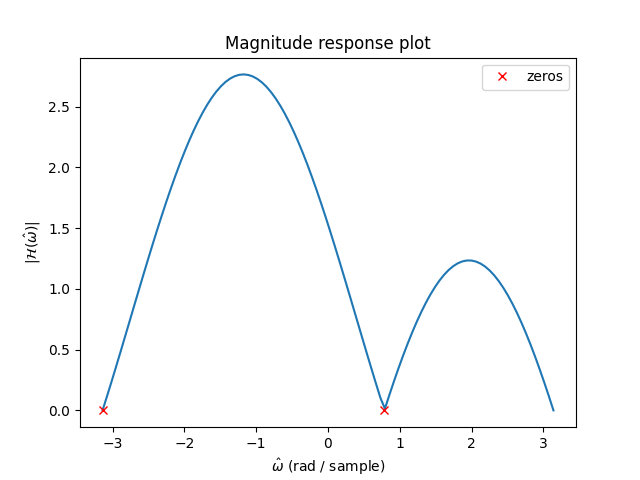
\includegraphics[width=7.5cm,height=7.0cm]{ch18/figures/magnituderes.png}
\caption{Plot of $|\mathcal{H}(\hat{\omega})|$, which has zeros at $\hat{\omega}=\pi/4$ and $\hat{\omega}=-\pi$.}
\label{h-plt}
\end{marginfigure}

\item The zeros of the magnitude response will get completely removed by the system. The original system has a system function $\mathcal{H}(z)$ which has two zeros, these being $\alpha_{1}=e^{i\pi/4}$ and $\alpha_{2}=e^{-i\pi}$. These correspond to $\hat{\omega}=\pi/4$ and $\hat{\omega}=-\pi$ in units of radians per sample. These discrete-time angular frequencies will be completely removed by the system. 

\item From the original definition of the system, we have:
\begin{align*}
    \mathcal{H}(z) &=(z-e^{i\pi/4})(z-e^{-i\pi})z^{-2}, \\
                   &=1-e^{i\pi/4}z^{-1}-e^{-i\pi}z^{-1}+e^{-i3\pi/4}z^{-2}, \\
                   &=1 -(e^{i\pi/4}+e^{-i\pi})z^{-1} + e^{-i3\pi/4})z^{-2}
\end{align*}
The non-zero values for $\beta{k}$ are $\beta_1=\alpha_{1}+\alpha_{2}$ and $\beta_2=\alpha_{1}\alpha_{2}$. 

\item To find the impulse response, we find the inverse $z$-transform of the system function. The impulse response $h[n]$ is then:
$$h[n]=\delta[n]-(e^{i\pi/4}+e^{-i\pi})\delta[n-1]+e^{-i3\pi/4}\delta[n-2]$$

\item For any discrete-time LTI system, we have:
$$y[n]=h[n]*x[n].$$
If the impulse response is real-valued, then the output signal will also be real-valued. If $h[n]$ is real-valued, it must satisfy: $h[n]^{*}=h[n]$. We can easily see that the impulse response doesn't satisfy this property, therefore a real-valued signal is not necessarily real-valued after applying this system. 

\end{enumerate}

\item Let $f_{s}=44.1\cdot 10^{3}$ Hz. 

\begin{enumerate}[a)]
\item To filter out the frequencies, we require that the system function has four zeros. These being at frequencies corresponding to $\pm5000$ and $\pm1500$ Hz. Thus, the system function will be a polynomial of degree four with four distinct roots. That is, the system function looks like:
$$\mathcal{H}(z)=(z-\alpha_1)(z-\alpha_2)(z-\alpha_3)(z-\alpha_4)$$
The frequencies in hertz corresponds to discrete-time angular frequencies of $\hat{\omega}_k=\omega T_s=2\pi f_k/fs$. This gives:
\begin{align*}
    \hat{\omega}_{0} &=  2\pi5000/44100 =  10\pi/441,\\
    \hat{\omega}_{1} &= -2\pi5000/44100 = -10\pi/441,\\
    \hat{\omega}_{2} &=  2\pi1500/44100 =  10\pi/147,\\
    \hat{\omega}_{3} &= -2\pi1500/44100 = -10\pi/147.
\end{align*}
Finally, the system function is therefore of the form:
\begin{align*}
    \mathcal{H}(z)&=(z-e^{10i\pi/441})(z-e^{-10i\pi/441})(z-e^{10i\pi/147})(z-e^{-10i\pi/147}), \\
    &=(1-e^{\frac{10\pi}{441}i}z^{-1})(1-e^{-\frac{10\pi}{441}i}z^{-1})(1-e^{\frac{10\pi}{147}i}z^{-1})(1-e^{-\frac{10\pi}{147}i}z^{-1})z^{4},\\
    &=(1-2\cos\left(\frac{10\pi}{441}\right)z^{-1}+z^{-2})(1-2\cos\left(\frac{10\pi}{147}\right)z^{-1}+z^{-2})z^{4}.
\end{align*}

\item A pole-zero diagram for the system function $\mathcal{H}(z)$ is shown in Figure \ref{z:ex4}.

\begin{marginfigure}[-5cm]
\begin{center}
\begin{tikzpicture}
	\begin{axis}[axis equal, ymin=-1.5,xmin=-1.5,ymax=1.5,xmax=1.5,  ticks=none,
    xlabel=$\mathrm{Re}(z)$,
    ylabel=$\mathrm{Im}(z)$, axis lines = middle, width=7cm, height=7cm]
	\addplot [gray,domain=0:2*pi,samples=50]({cos(deg(x))},{sin(deg(x))});

\addplot [blue, mark = o,mark size=3pt] coordinates {({cos(40)}, {sin(40)})} {};  
\addplot [blue, mark = o,mark size=3pt] coordinates {({cos(-40)}, {sin(-40)})} {};   
\addplot [blue, mark = o,mark size=3pt] coordinates {({cos(12.2)}, {sin(12.2)})} {};  
\addplot [blue, mark = o,mark size=3pt] coordinates {({cos(-12.2)}, {sin(-12.2)})} {};  
\addplot [red, mark = x,mark size=3pt] coordinates {({0}, {0})} {}; 
\end{axis}
\end{tikzpicture}
\end{center}
\caption{The zeros of the system function $\mathcal{H}(z)$,
have $\alpha_k=\{e^{10i\pi/441},e^{-10i\pi/441},e^{20i\pi/441},e^{-20i\pi/441}\}$. Zeros are marked with blue circles and poles are marked with red crosses.}
\label{z:ex4}
\end{marginfigure}

\item Listing \ref{z:code:ex4} provides code to plot the magnitude response for this system.

\begin{lstlisting}[language=Python,caption=Code to plot the magnitude response,label=z:code:ex4]
import numpy as n
import matplotlib.pyplot as plt

# function to convert to dB
def convert_to_decibel(x):
    return 10*n.log10(n.abs(x)**2)

# partition the interval (-pi,pi)
om = n.linspace(-n.pi,n.pi,num=10000)

# definition of the system function, H(z):
def system_function(z):
    return (1 - n.exp(1j*100*n.pi/441)*z**(-1))*(1 - n.exp(-1j*100*n.pi/441)*z**(-1))*(1 - n.exp(20*1j*n.pi/441)*z**(-1))*(1 - n.exp(-20*1j*n.pi/441)*z**(-1))*z**4

# frequency response
def frequency_response(om):
    return system_function(n.exp(1j*om))

# plot the system function with the zeros marked
plt.plot(om,convert_to_decibel(frequency_response(om)),label="$\mathcal{H}(\hat{\omega})$")
plt.xlabel("$\hat{\omega}$ (rad / sample)")
plt.ylabel("$|\mathcal{H}(\hat{\omega})|$")
plt.title("Magnitude response plot")
plt.legend()
plt.show()
\end{lstlisting}
Output of Listing \ref{z:code:ex4} is shown in Figure \ref{z:fig:ex4}.

\begin{marginfigure}
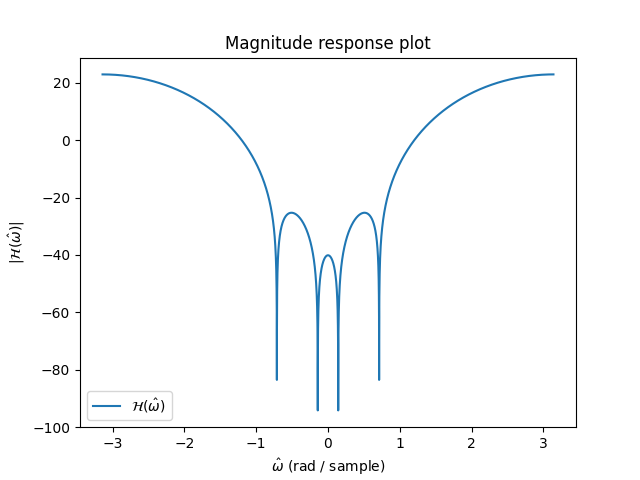
\includegraphics[width=7.5cm,height=7.0cm]{ch18/figures/mag2.png}
\caption{Plot of the magnitude response in dB}
\label{z:fig:ex4}
\end{marginfigure}

\item Having found the system function, one can easily determine the impulse response function by using the inverse $z$-transform. Have that:
\begin{align*}
    \mathcal{H}(z)&=(1-2\cos\left(\frac{10\pi}{441}\right)z^{-1}+z^{-2})(1-2\cos\left(\frac{10\pi}{147}\right)z^{-1}+z^{-2})z^{4}. 
\end{align*}
Expanding all of this out, one obtains:
\begin{align*}
    \mathcal{H}(z)&=z^{4} -2(\cos(\theta_1)+\cos(\theta_2))z^{3} + 2(2\cos\theta_1\cos\theta_2 + 1)z^{2} -2(\cos\theta_1+\cos\theta_2) z + 1,
\end{align*}
where $\theta_1=\frac{10\pi}{441}$ and $\theta_2=\frac{10\pi}{147}$. The impulse response is then the inverse $z$-transform:
$$h[n]=\delta[n]-2(\cos\theta_1+\cos\theta_2)\delta[n-1]+2(2\cos\theta_1\cos\theta_2+1)\delta[n-2]-2(\cos\theta_1+\cos\theta_2)\delta[n-3]+\delta[n-4].$$




\end{enumerate}




\end{enumerate}